\begin{frame}{Work on Application Code for X-ray Imaging at USC/ISI} 
\begin{enumerate} 
\item Performance assessment 
\begin{itemize} 
\small \item \small Computational requirements to calculate number of GPUs needed. 
\item \small Ensured that a dedicated network, similar to ESnet, doesn’t slow down computation: our application has unique requirements in that we need to stream the input data from data source to the supercomputer center.
\end{itemize}
\item Performance optimization.
\begin{itemize} 
\small \item \small Ptychography code optimization: compiler flag optimization, loop unrolling, started work on half-precision instructions for NVIDIA Tesla P100.
\item \small Tomography code optimization: discussed and worked on translating matlab code to C++ code, including working on numerical optimization.
\end{itemize}
\item Procurement of resources to set up experiments.
\begin{itemize}
\small \item \small Obtained machine resources from University of Southern California's High Performance Computing Center.
\small \item \small Worked on proposal for Intel MICs to add to USC HPC system.
\end{itemize}
\end{enumerate}
\end{frame} 

\begin{frame}{What We Are Trying To Do}
\begin{enumerate} 
\item Overview of problem/solution: Image reconstruction of 3-d chip : explain problem from Broad Agency Announcement. 
\item Implementation details of problem/solution: Figure of overall problem: 
\item Coherent Diffraction Imagery:  
\begin{itemize} 
\small \item \small 2-dimensional Reconstruction:  ptychography 
\item \small 3-dimensional reconstruction from slices generated by ptychography using tomography algorithms. 
\end{itemize} 
\end{enumerate}
\begin{figure}[ht!]
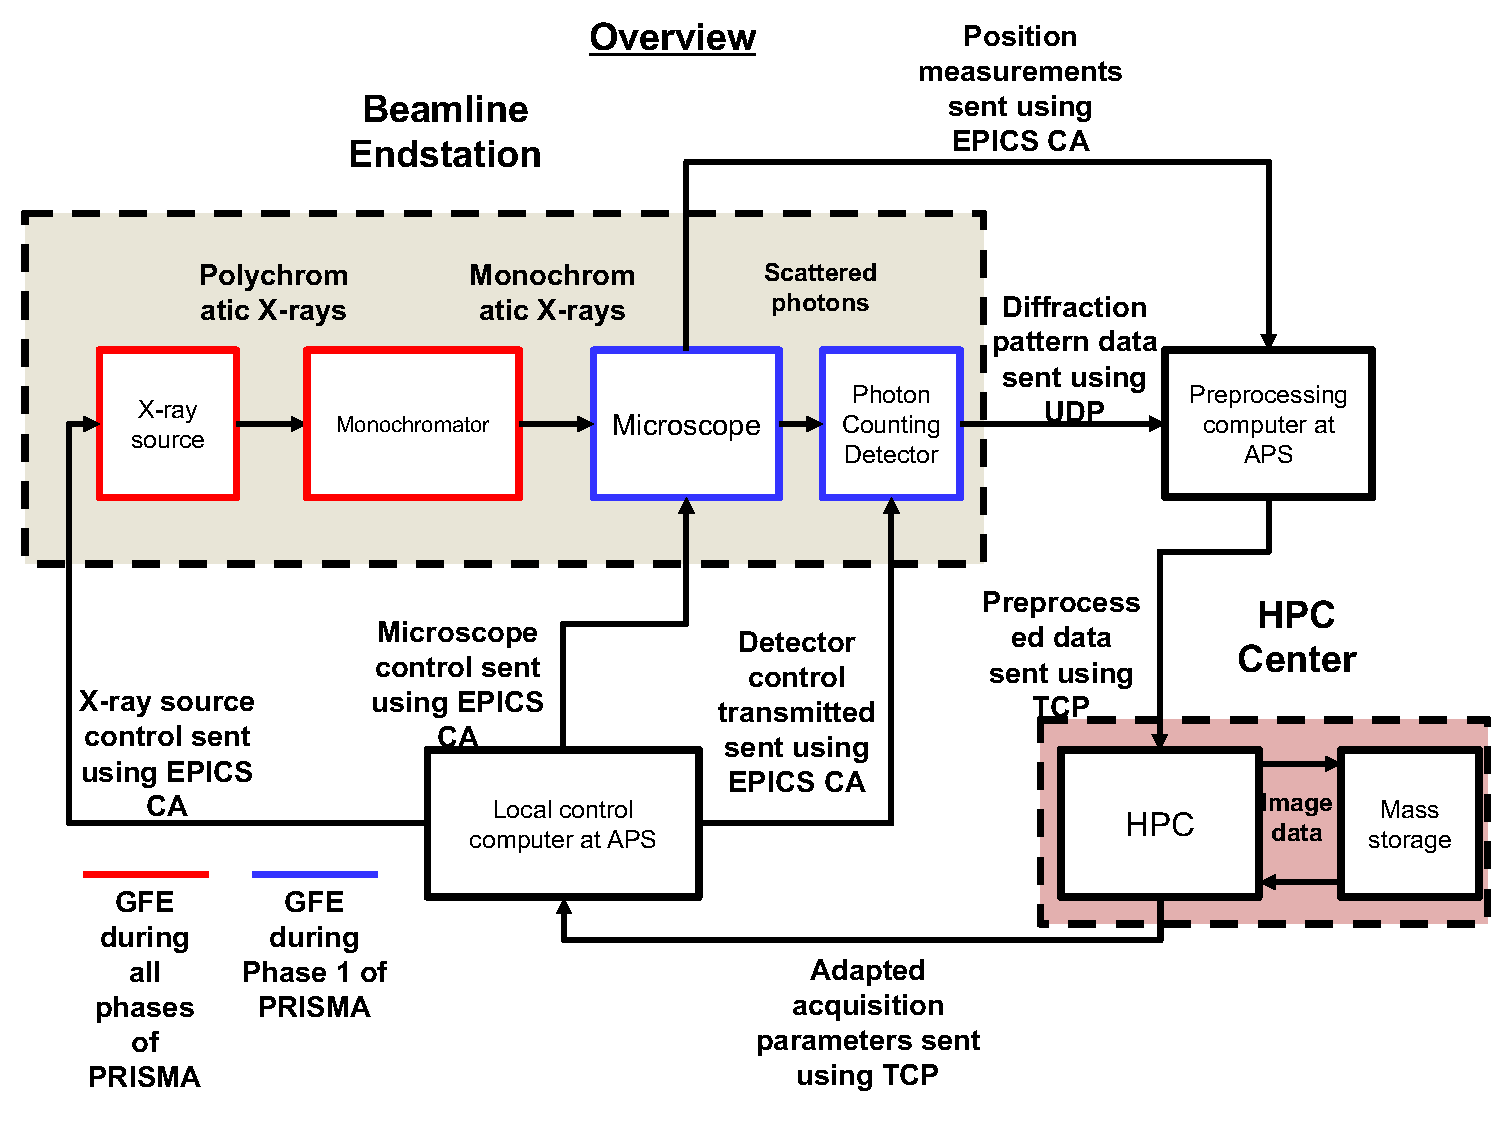
\includegraphics[scale=0.22]{./images/exp_schematic_1017_1}
\end{figure} 
\end{frame}

\begin{frame}{Computational Aspects of Problem} 
\begin{figure}[ht!]
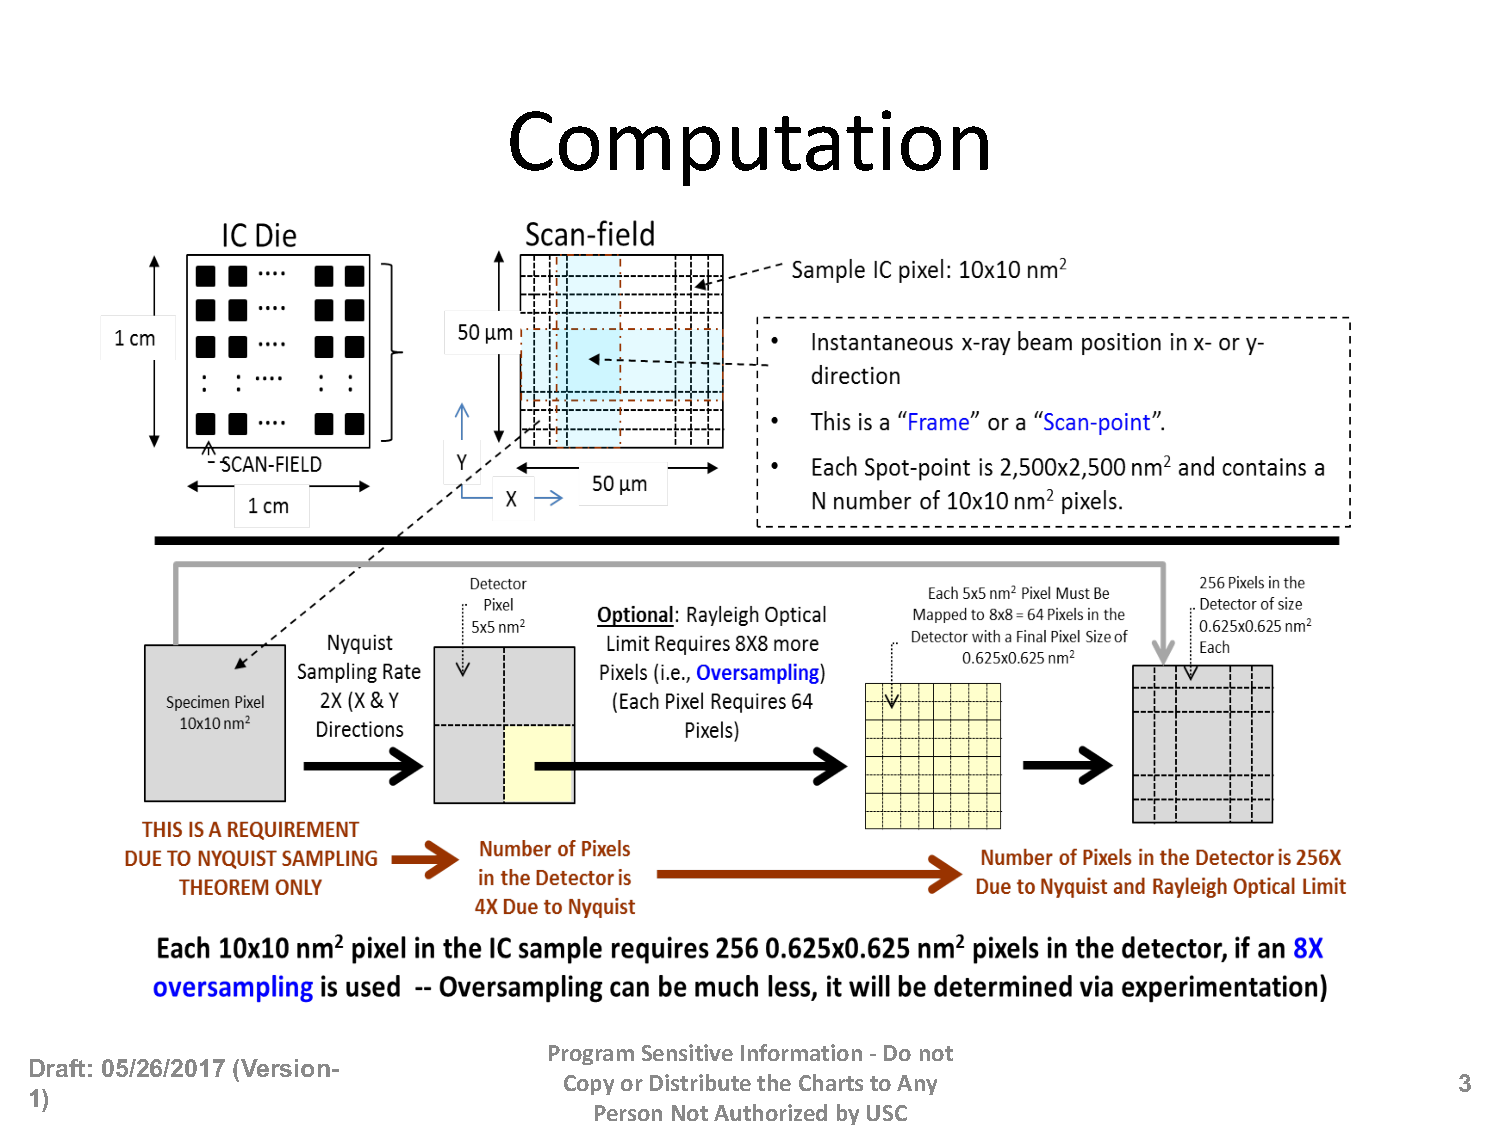
\includegraphics[scale=0.4]{./images/exp_schematic_1017_2}
\end{figure}
\end{frame}

\begin{frame}[label=AppUnderstanding]
\frametitle{Understanding Numerical Algorithm}
{\small \underline{\bf X-ray Imaging Algorithms}}
\begin{itemize}
\tiny \item \tiny Use ePIE due to memory footprint of DM. DM uses 5 GB because it stores buffers for current and previous wavefront while ePIE uses 1 GB.
\tiny \item \tiny ePIE tries to recover two distinct quantities: (1)
the probe wavefront describing the beam incident on a sample and (2) the object transmission function describing the sample under
investigation.
\end{itemize}
{\small \underline{\bf Code}}
\begin{itemize}
\item \tiny ePIE is embarassingly parallel with collective communication at the end.
\item \tiny Updates the object and probe function on each iteration.
\item \tiny Steps to update the object and probe function are repeated for every diffraction pattern j and for a number of ePIE iterations, or until a certain convergence criterion is met.*
\end{itemize}
{\small \underline{\bf Performance Optimizations}}
\begin{itemize}
\tiny \item \tiny Uses NVIDIA cuFFT library for optimization of FFT calculations.
\item \tiny Uses DIY library for partitioning of data across nodes.
\item \tiny Uses memory coalescing on GPU and partitioning of data onto GPU for load balancing.
\end{itemize}
{\tiny \textit{Parallel Ptychographic Reconstruction. Nashed et al.}}
\end{frame}

\begin{frame}{Procurement of Resources to Set Up Experiments} 
\begin{enumerate} 
\item Obtained GPU machine resources from USC HPC
\begin{itemize}
\small \item \small Focused on applications for ptychography, which is
a compute-intensive code with same work repeated across outer loop
iterations. 
\small \item \small Benchmarking. 
\end{itemize}
\item Worked on proposal for Intel MICs to add to USC HPC system.
\begin{itemize} 
  \small \item \small Justified adding Intel Xeon Phi to existing HPC
  system to run experiments of OpenMP-ized version of the code. 
\end{itemize} 
\item Worked on network infrastructure. 
\begin{itemize} 
\item \small benchmarking to know existing capabilities.
\item \small Burst buffers. 
\item \small Provisioning. 
\end{itemize}
\end{enumerate}
\end{frame} 

\begin{frame}{Performance Assessment}
\begin{enumerate}
\item Performance Profiling
\begin{itemize}
\item Used CUDA PAPI to profile cache misses of MPI+CUDA, leads to work on roofline model.
\item Looked into call-path + causal profiling for MPI+CUDA for identifying where FFTs are called. 
\item Looked at tomography code performance to project number of GPUs needed. 
\end{itemize} 
\item Performance Modeling
\begin{itemize}
\item Computational requirements to calculate number of GPUs needed. 
\item Ensured that a dedicated network, similar to ESnet, doesn’t slow down computation: our application has unique requirements in that we 
  need to stream the input data from data source to the supercomputer center. 
\end{itemize} 
\end{enumerate} 
\end{frame} 

\begin{frame}[label=scalingptycho]{Performance Modeling of Computation}
\begin{itemize}
\tiny \item \tiny 
\item \tiny 
\end{itemize} 
\begin{figure}[ht!]
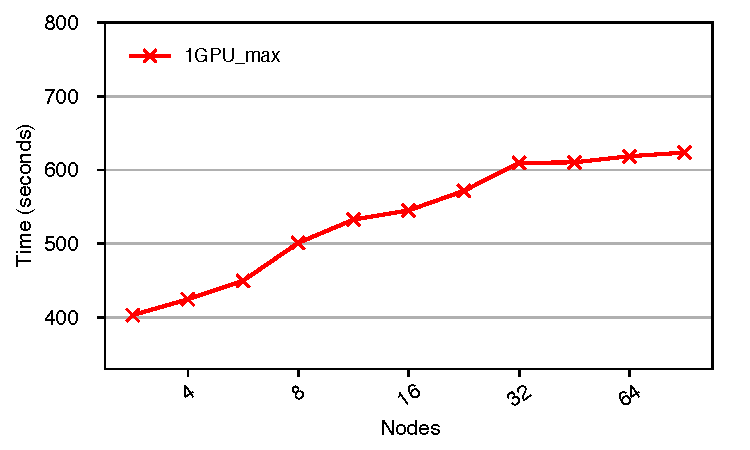
\includegraphics[scale=0.5]{./plots/ptychoLib-hpcc-weakscale-intro.pdf}
\end{figure}
\underline{\bf Timings for Tomography:} 1 CPU with full problem size:
20 seconds, 1 MPI process '' '': 12.0 seconds , 16 MPI processes: 2.75 seconds 
\underline{\bf Timings for Tomography(weak Scale):} 32 MPI processes
on two nodes: 3.34 seconds | 64 MPI processes on 4 nodes: 4.10 seconds 

%\begin{figure}[ht!]
%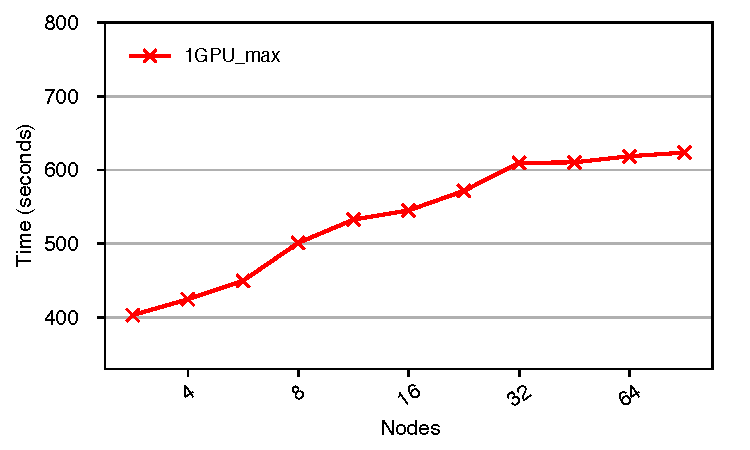
\includegraphics[scale=0.5]{./plots/ptychoLib-hpcc-weakscale-intro.pdf} 
%\end{figure} 
\begin{enumerate}
\tiny \item \tiny 
\item \tiny 
\end{enumerate}
\end{frame}


\comments{ 
\begin{frame}[label=mpicudaprofile]{MPI+CUDA Call-path and Causal Profiling}
\end{frame}

\begin{frame}[label=mpicudaprofile]{MPI+OpenACC NAS Benchmarks}
\end{frame} 

}


\begin{frame}{Performance Optimizations}{} 
\begin{enumerate}
\item Ptychography code optimization.
\begin{itemize}
\small \item \small compiler flag optimization.
\item \small loop unrolling. 
\item \small started work on half-precision instructions for NVIDIA Tesla P100. 
\end{itemize}
\item Tomography code optimization. 
\begin{itemize} 
\small \item \small discussed and worked on translating matlab code to C++ code.
\item \small including working on numerical optimization.
\end{itemize}
\item Input data transfers. 
\begin{itemize} 
\small \item \small Compression of data. 
\item \small Middleware for data storage, e.g., HDF5 .  
\end{itemize} 
\end{enumerate} 
\end{frame}


\comments{
\begin{frame}{Performance Optimization of Ptychography Code}{Using Half-precision Instructions} 
%\begin{lstlisting}
%\lstinputlisting{./listings/halfPrecisionCodeSnippet.cc}
%\end{lstlisting}
\end{frame}

\begin{frame}{Performance Optimization of Ptychography Code}{Compiler Optimizations and Loop Unrolling} 
\end{frame} 
}

\begin{frame}{Results of Performance Optimization of Ptychography Code}
\begin{itemize}
\item Using loop transformations on a variety of compiler flag optimizations on the ptychoLib code improves performance of the
ptychoLib code by 12.2\%. 
\item Using Tesla P100 half-precision instructions on code
  representative of PtychoLib improves performance of the code by
  13.2\% (--TODO: check this through back-of-envelope calcs--)
\end{itemize}
\end{frame}

\comments{
\begin{frame}{Performance Optimization of Tomography Code}{Using MPI C++ instead of MATLAB}
\begin{figure}
    \centering
 \lstinputlisting{./listings/tomographyCode.cc}
    \caption{Code for Tomography}
    \label{fig:my_label}
\end{figure}
\end{frame} 

\begin{frame}{Performance Optimization of Tomography Code}{Numerical Algorithm and Memory Optimization}
\begin{figure}
    \centering
\lstinputlisting{./listings/tomographyCode2.cc}

    \caption{}
    \label{fig:my_label}
\end{figure}
\end{frame} 

\begin{frame}{Results of Performance Optimization for Tomography Code}
  \begin{itemize}
    \tiny \item \tiny  Average of 1.49 seconds. Std deviation: 0.02 seconds. Over 5 trials.
  \end{itemize}
\end{frame} 

}


\comments{
\begin{frame}[label=proposalTimeAlloc]
\frametitle{Proposal for Parallel Machine Time Allocation}
%Application for access to USC compute resources.% 

\begin{outline}[enumerate]
\tiny \1 {\tiny Context and Goal}
\tiny \2 {\tiny Context: need to better understand behavior of
  Integrated Circuits(IC)/computer chips technology to make
  advancements IC technology.}
\tiny \2 {\tiny Goal: Construct an image to simulate operation of
  integrated circuit.}
\tiny \3 {\tiny The following requirements for image reconstruction
are needed: Real-time feedback during imaging, use of x-ray sources,
establish highly reliable program.}
\tiny \1 {\tiny Project Methodology: How will you proceed? What kind
of data or software will you use or install?}
\tiny \2 {\tiny Use Ptychography technique to generate a 2D image and
  then use tomography to combine the 2D images to 3D images.}
\tiny \2 {\tiny Data and Software:}
\tiny \3 {\tiny software: Ptycholib for constructing ptycholib algorithms.}
\tiny \3 {\tiny For data for doing experimentation, we'll use Argonne's advanced photon source.}
\tiny \1 {\tiny Justification: (How will HPC use improve your results and help acheive your goals)}
\tiny \2 {\tiny Ptychography is computationally intensive with FFTs. }
\tiny \2 {\tiny GPU resources allow for throughput computing and will
  help improve efficiency of our simulations.}
\tiny \2 {\tiny interconnect network of cluster will help to improve efficiency of FFT algorithms.}
\2 {\tiny The improvements in efficency can help with doing more
scientific calculations per second so as to allow for achieving high
resolution images and satisfying the three requirements described in
the response of the prompt Project Methology.} 
\end{outline}

\end{frame}  

}
